\section{Bestiario delle Ere
Primordiali}\label{bestiario-delle-ere-primordiali}

\begin{quote}
Nel crepuscolo dei tempi, quando Astarte era un mosaico di poteri divini
e la creazione danzava sulla soglia dell'eternità, nacquero creature
destinate a incarnare la magnificenza primordiale. Questo Bestiario
delle Ere Primordiali è un monumento eretto dalla perseveranza di
decenni di pellegrinaggi, una testimonianza di ciò che fu un tempo e di
ciò che ancora persiste nell'eco delle leggende. Questo Bestiario delle
Ere Primordiali è il frutto di decenni di pellegrinaggi attraverso terre
remote, un'epopea di conoscenza raccolta ascoltando antiche leggende e
recuperando informazioni ormai perdute nei meandri del tempo. Qui, tra
le pagine di questo tomo, si svelano le immagini delle bestie ancestrali
che un tempo solcavano i cieli di Astarte, calpestavano le sue terre
selvagge e dominavano gli abissi del suo regno marino. Ogni creatura
narrata in queste pagine è un frammento del passato primordiale, una
testimonianza vivente delle forze che plasmarono il mondo nei suoi
albori. Nel corso di innumerevoli pellegrinaggi attraverso montagne
antiche, foreste impenetrabili e deserti eterni, gli studiosi hanno
ascoltato le voci del passato che sussurrano ancora nel vento. Le
leggende tramandate da generazioni hanno trovato rifugio in queste
pagine, creando un ricamo di verità e mito intrecciato con maestria.
Ogni descrizione è un rituale di evocazione delle creature primordiali,
una chiamata ai tempi in cui gli dèi stessi intessero la trama della
creazione. Che tu sia un viandante curioso o uno studioso desideroso di
scrutare gli archivi dell'antichità, il Bestiario delle Ere Primordiali
è la tua chiave per penetrare il velo del passato e immergerti nelle
storie delle creature che un tempo furono padrone indiscusso di Astarte.
Che questa opera ti guidi attraverso le epoche, portandoti più vicino a
comprendere l'essenza stessa delle Ere Primordiali. - Fra' Antonius Rixi
\end{quote}

\subsection{Drago Rosso}\label{drago-rosso}

\begin{figure}
\centering
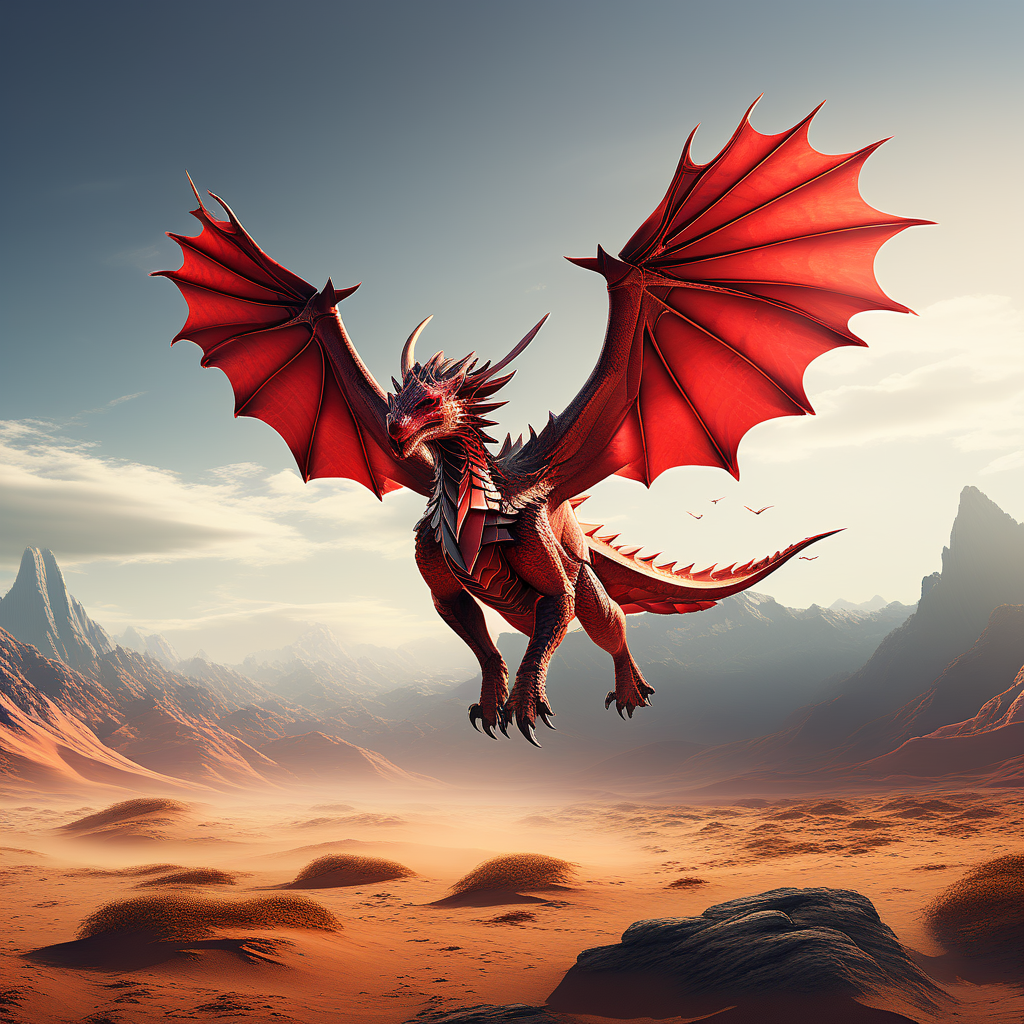
\includegraphics{create-an-image-of-a-red-dragon-flying-over-a-desert-with-the-stylised-style-of-medieval-bestiaries-.png}
\caption{create-an-image-of-a-red-dragon-flying-over-a-desert-with-the-stylised-style-of-medieval-bestiaries-.png}
\end{figure}

Il drago rosso, incarnazione del fuoco, si erge con imponente
maestosità. La sua corazza di scaglie rosse, simili a lingue di fiamma,
riflette l'intensa forza che lo abita. Le ali membranose, sostenute da
ossa dorate, brillano con una luce arancione dorata. Gli occhi infuocati
sfoggiano astuzia e saggezza ancestrali. Il ruggito, un tuono di fuoco,
segna la sua supremazia. Le zampe artigliate e possenti, come uncini
ardenti, testimoniano la sua regalità tra i draghi. Una creatura
magnifica e spaventosa, il drago rosso incarna la potenza distruttiva
del fuoco.

\subsection{Drago Bianco}\label{drago-bianco}

Il drago bianco, sovrano delle regioni glaciali, si presenta con
eleganza maestosa. La sua pelle di scaglie ghiacciate, bianca come la
neve, brilla sotto la luce lunare. Le ali membranose, attraversate da
venature bluastre, sembrano dipinte dall'inverno eterno. Gli occhi
azzurri, freddi come il ghiaccio, rivelano una ferma intelligenza. Il
suo ruggito, un vento gelido, echeggia tra le vette montuose. Le zampe
possenti, artigliate come ghiacci affilati, attestano la sua regalità
tra i draghi. Il drago bianco incarna la potenza glaciale, una creatura
sublime e temibile.

\begin{figure}
\centering
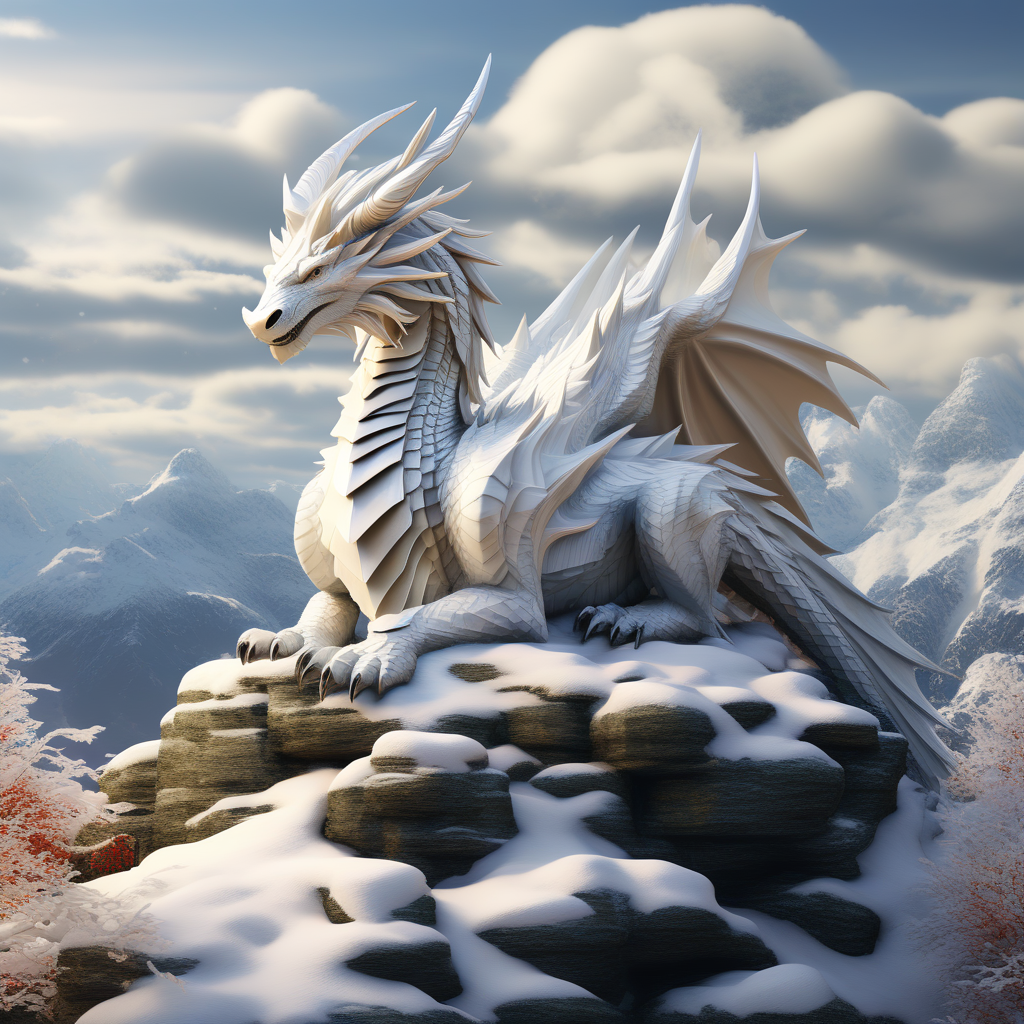
\includegraphics{create-an-image-of-a-white-dragon-resting-on-top-of-a-snowy-mountain-with-the-stylised-style-of-medi-2.png}
\caption{create-an-image-of-a-white-dragon-resting-on-top-of-a-snowy-mountain-with-the-stylised-style-of-medi-2.png}
\end{figure}

\subsection{Kraken}\label{kraken}

\begin{figure}
\centering
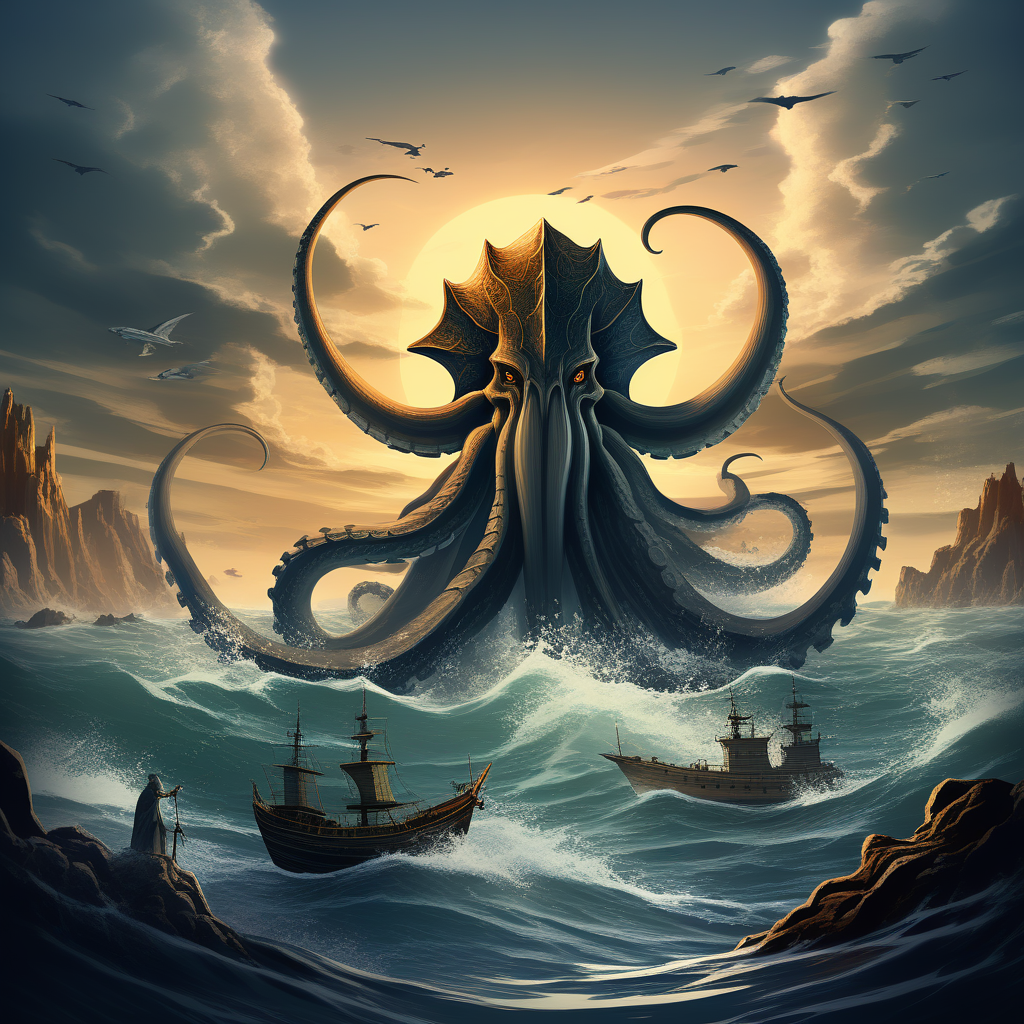
\includegraphics{create-an-image-of-a-kraken-roaming-the-sea-with-the-stylised-style-of-medieval-bestiaries--2.png}
\caption{create-an-image-of-a-kraken-roaming-the-sea-with-the-stylised-style-of-medieval-bestiaries--2.png}
\end{figure}

Il Kraken, terrore degli abissi, è una creatura marina leggendaria di
proporzioni gigantesche. La sua massa oscura e squamosa si staglia
contro il cielo d'azzurro, mentre tentacoli corazzati e sottili si
estendono dalla superficie dell'acqua, pronti a trattenere e affondare
qualsiasi nave sventurata che attraversi il suo territorio. Gli occhi
enormi e luminescenti fissano gli intrusi con un'intelligenza antica,
emanando una luce blu profonda. La sua presenza è accompagnata da
un'aura di potere, facendo sì che il mare stesso si ritiri timoroso di
fronte a questa creatura colossale.

\subsection{Sandworm}\label{sandworm}

Il Verme del Deserto, colosso delle dune, si insinua nell'aridità con
maestosità spietata. La sua pelle squamosa, dai toni del deserto, si
camuffa con l'ambiente sabbioso. Mascelle possenti, punteggiate di denti
affilati, svelano la sua natura predatrice. Gli occhi, brillanti di una
luce dorata, scrutano l'orizzonte mentre emerge dalla sabbia. Dotato di
agilità sorprendente sotto terra, il Verme del Deserto colpisce con
attacchi fulminei, catturando chiunque sfidi il suo dominio. La sua
coda, come un tornado di sabbia, è un'arma temibile. Il Verme del
Deserto, narrato tra i viaggiatori, è il terrore delle terre brucianti.

\begin{figure}
\centering
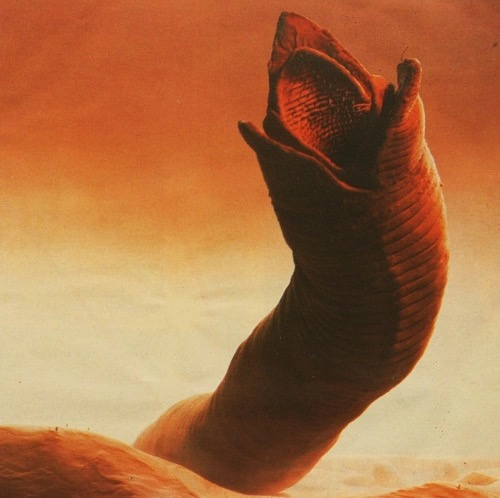
\includegraphics{sandwormcropped.jpg.webp}
\caption{sandwormcropped.jpg.webp}
\end{figure}

\subsection{Besugus}\label{besugus}

\begin{figure}
\centering

\includegraphics{artworks-yPCycR4TUZ9Tk0BK-omHBMw-t500x500.jpg}
\caption{artworks-yPCycR4TUZ9Tk0BK-omHBMw-t500x500.jpg}
\end{figure}

Il Besugus, creatura delle oscure foreste, si cela nell'ombra con la sua
pelle rossa sanguigna e la testa mostruosa. Dotato di occhi sinistri e
un sorriso distorto, Besugus caccia in branco con un ghignante richiamo
di besugi e un ululato inquietante. Le sue zampe artigliate e snodabili
muovono l'animale con una sinistra agilità, mentre il suo habitat, un
luogo di risate irreali e grida spettrali, diventa il teatro di
cacciatori notturni. Nelle tenebre delle sue foreste, Besugus incute
timore, un orrore incarnato dalle sue movenze e dal suo sguardo
famelico.

\subsection{Roc}\label{roc}

Il Roc, signore etereo dei cieli, spande le ali tese come un mantello
d'azzurro tempestoso. Il suo piumaggio, sfumato di blu e argento, evoca
l'iridescenza di un cielo stellato. Con l'apertura alare che oscura il
firmamento, il Roc plana, imponente e regale. Il becco affilato come una
lama traccia linee imperiose nell'aria, mentre gli occhi scrutano il
mondo dall'alto. Zampe possenti, artigli come fulmini, testimoniano il
dominio incontrastato del Roc nei cieli. Nella mitologia, il suo volo è
un'ode al divino, un'epopea silenziosa di forza e maestosità che pervade
i reami celesti.

\begin{figure}
\centering
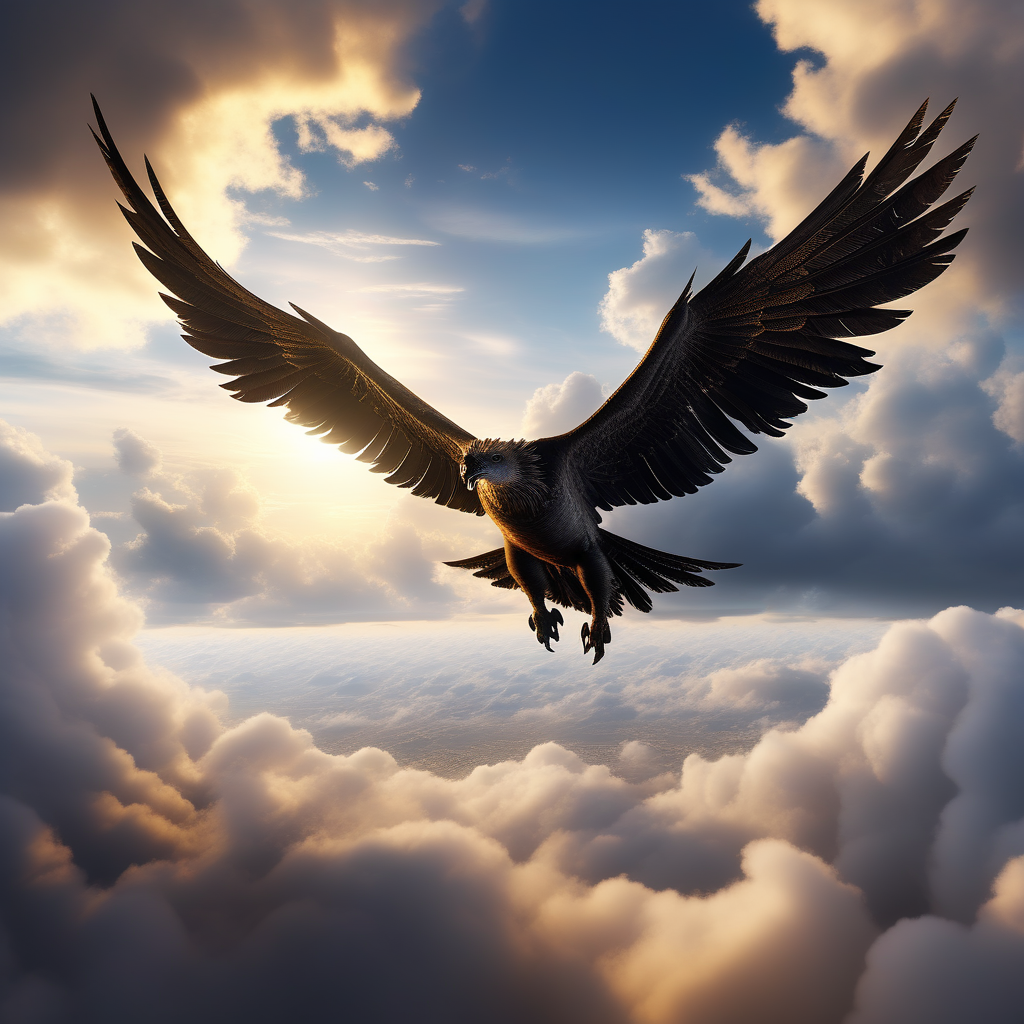
\includegraphics{a-giant-roc-flying-up-in-the-sky-his-silhouette-hidden-in-the-clouds-bottom-up-perspective-perfec.png}
\caption{a-giant-roc-flying-up-in-the-sky-his-silhouette-hidden-in-the-clouds-bottom-up-perspective-perfec.png}
\end{figure}

\subsection{Idra}\label{idra}

\begin{figure}
\centering
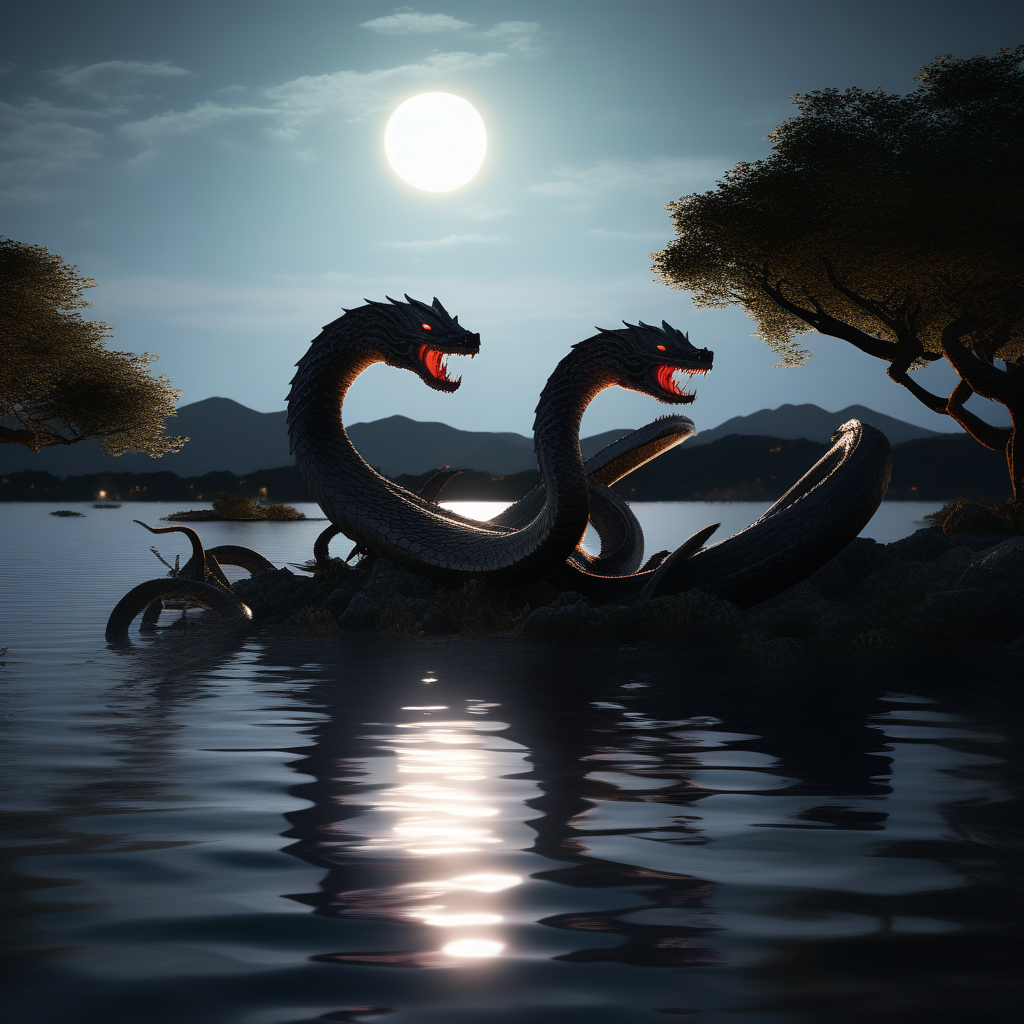
\includegraphics{an-hydra-emerging-from-a-lake-at-night-a-full-moon-on-the-background-shines-on-the-scene-perfect-c.png}
\caption{an-hydra-emerging-from-a-lake-at-night-a-full-moon-on-the-background-shines-on-the-scene-perfect-c.png}
\end{figure}

L'Idra, serpente delle acque oscure, incute terrore con la sua
molteplicità. Le scaglie risplendono sotto la luce lunare, svelando un
corpo snodato che si insinua sinistramente attraverso fiumi e stagni. Le
teste, numerose e sempre rinnovate, si ergono su colli serpentini, occhi
che bramano la preda con ossessione. Le fauci gocciolanti, imbevute di
veleno, sibillano morte mentre l'Idra cattura ogni cosa nel suo raggio
d'azione. Code serpeggianti radicate nelle profondità fungono da
tentacoli insidiosi. L'Idra, incarnazione del caos, risorge con potenza
maggiore ad ogni scontro, una minaccia che emerge dall'oscurità delle
acque.

\subsection{Galleria Immagini}\label{galleria-immagini}

\begin{figure}
\centering
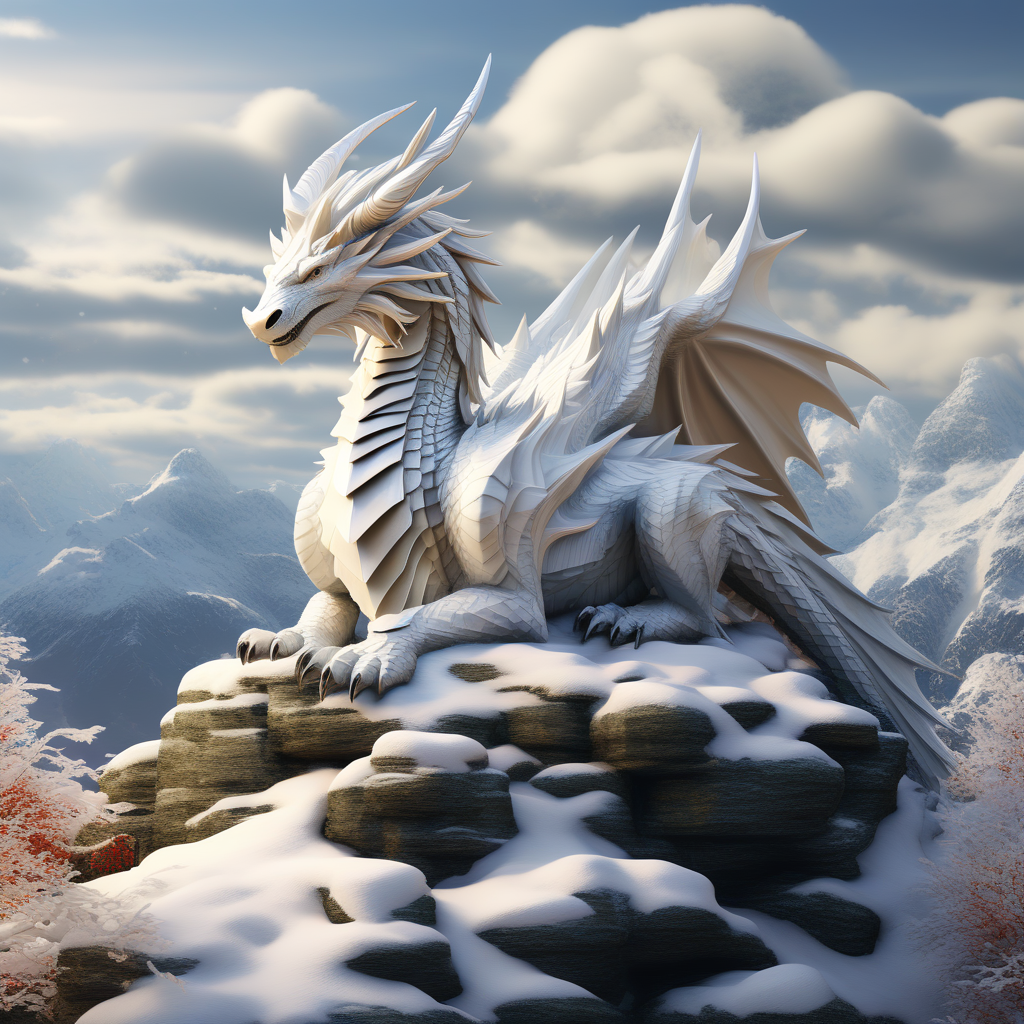
\includegraphics{create-an-image-of-a-white-dragon-resting-on-top-of-a-snowy-mountain-with-the-stylised-style-of-medi-2 1.png}
\caption{Drago Bianco}
\end{figure}

Drago Bianco

\begin{figure}
\centering
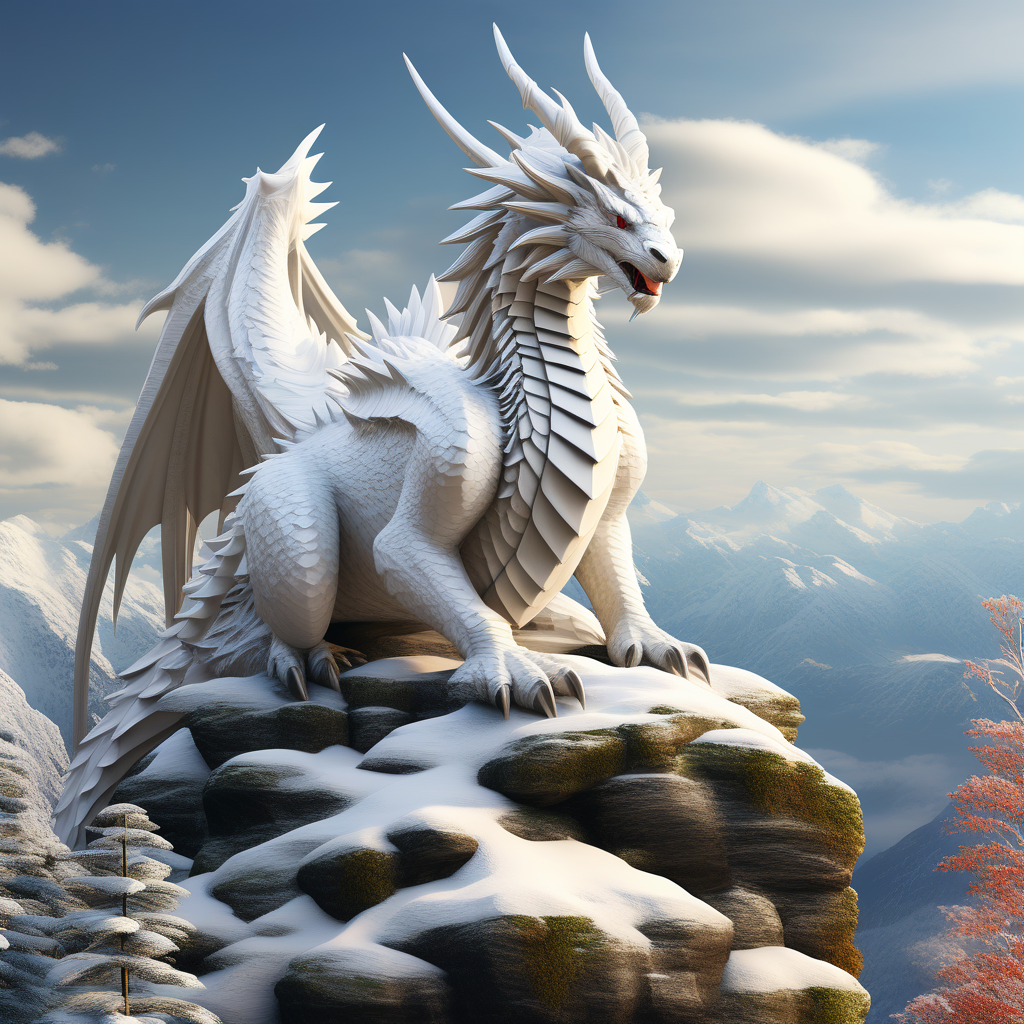
\includegraphics{create-an-image-of-a-white-dragon-resting-on-top-of-a-snowy-mountain-with-the-stylised-style-of-medi.png}
\caption{Drago Bianco}
\end{figure}

Drago Bianco

\begin{figure}
\centering
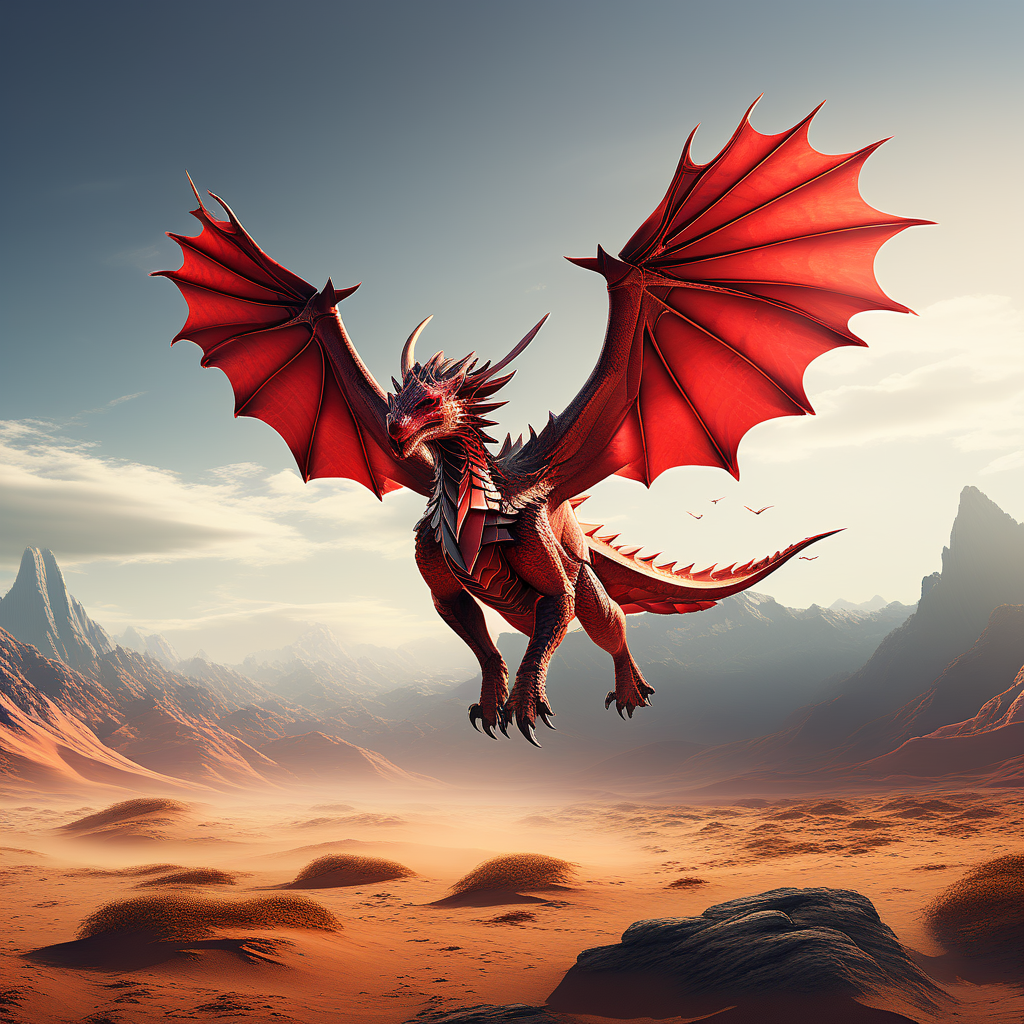
\includegraphics{create-an-image-of-a-red-dragon-flying-over-a-desert-with-the-stylised-style-of-medieval-bestiaries- 1.png}
\caption{Drago Rosso}
\end{figure}

Drago Rosso

\begin{figure}
\centering
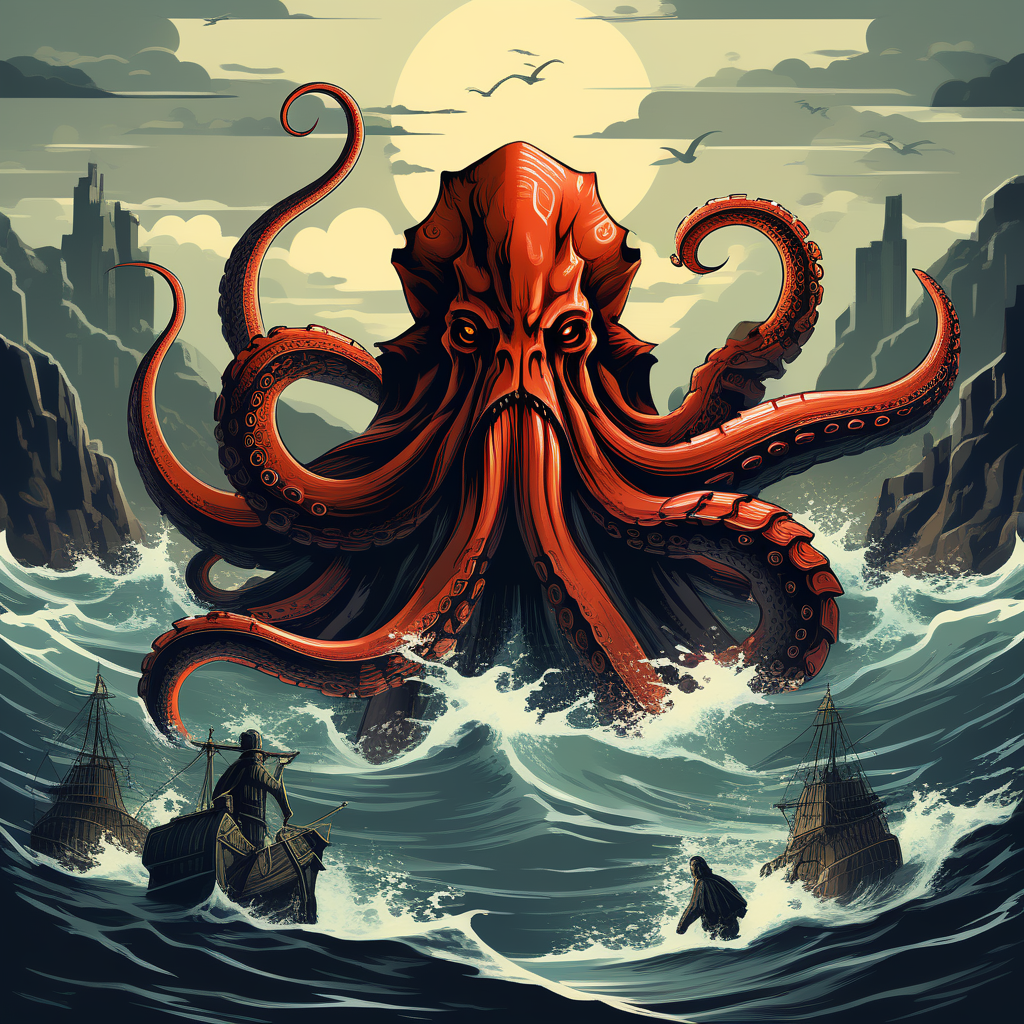
\includegraphics{create-an-image-of-a-kraken-roaming-the-sea-with-the-stylised-style-of-medieval-bestiaries-.png}
\caption{Kraken}
\end{figure}

Kraken

\begin{figure}
\centering
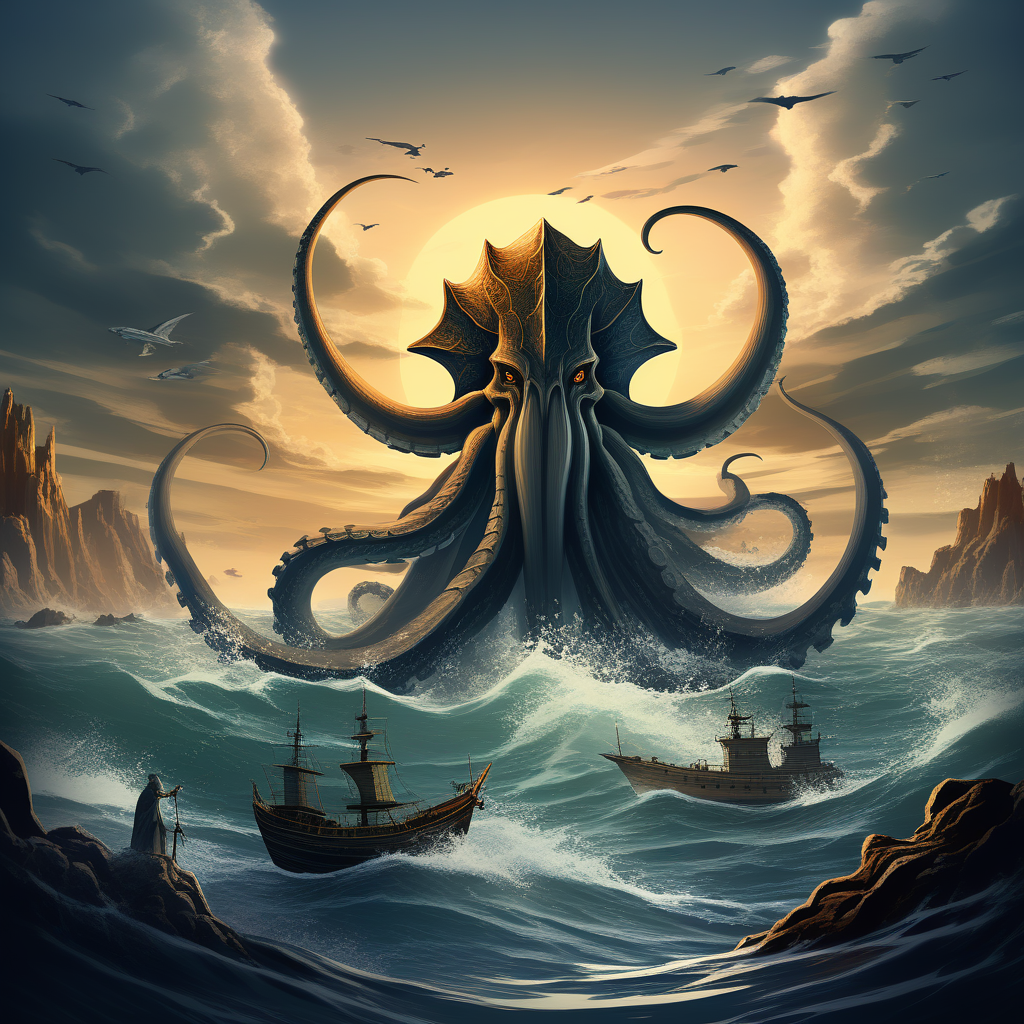
\includegraphics{create-an-image-of-a-kraken-roaming-the-sea-with-the-stylised-style-of-medieval-bestiaries--2 1.png}
\caption{Kraken}
\end{figure}

Kraken

\begin{figure}
\centering
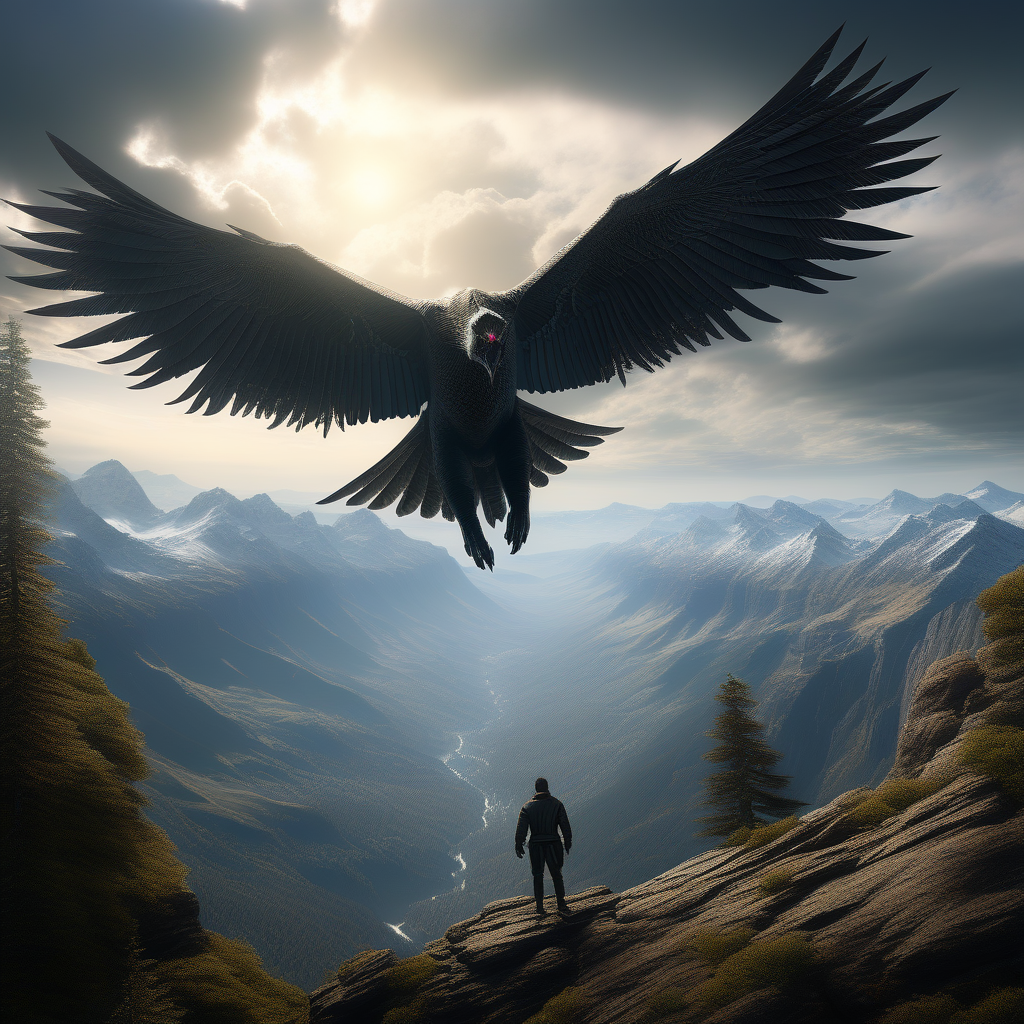
\includegraphics{a-giant-roc-flying-over-the-rocky-mountains-his-shadow-covers-most-of-the-landscape-sf-intricate-.png}
\caption{Roc}
\end{figure}

Roc

\begin{figure}
\centering
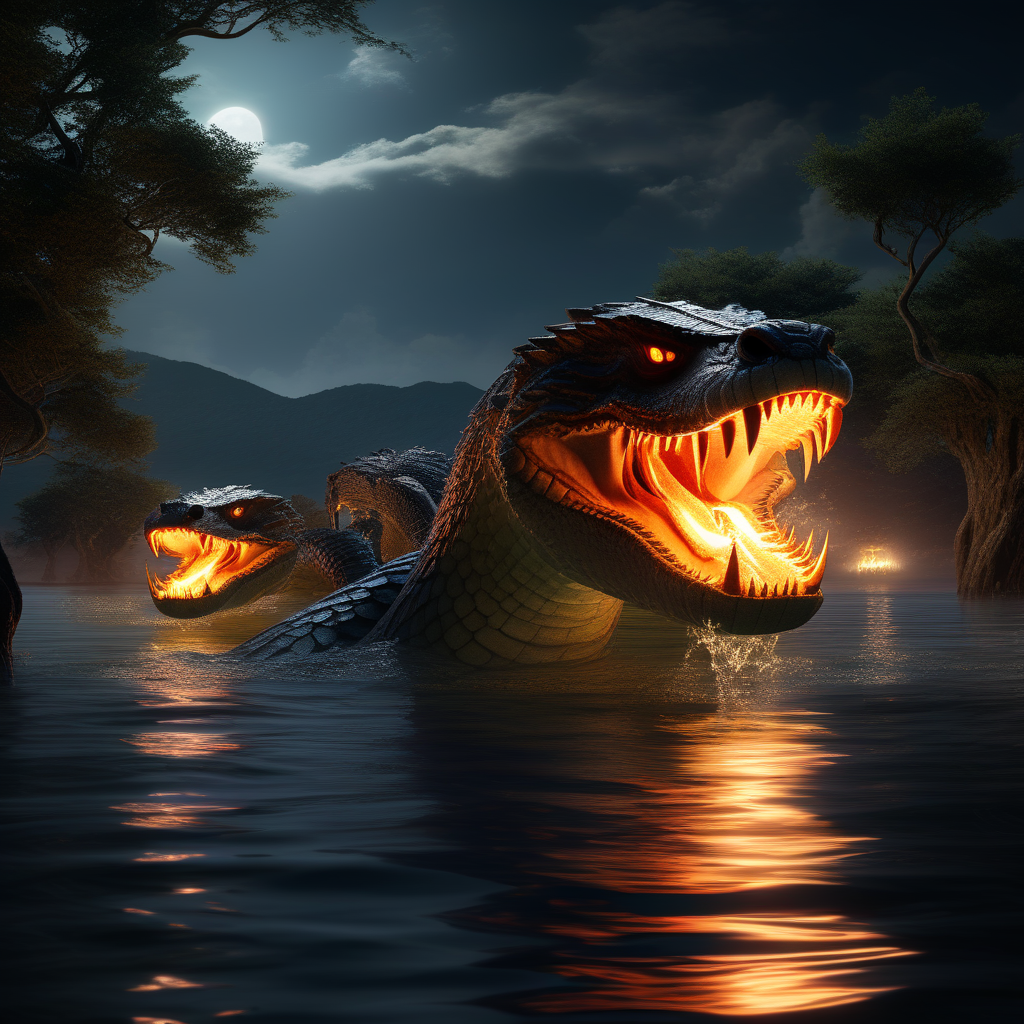
\includegraphics{an-hydra-emerging-from-a-lake-at-night-with-its-7-heads-a-full-moon-on-the-background-shines-on-th.png}
\caption{Idra}
\end{figure}

Idra
